\documentclass[aspectratio=169]{beamer}

\usetheme{Madrid}
\usecolortheme{default}
\usefonttheme{professionalfonts}

\usepackage[spanish, es-nodecimaldot]{babel}
\usepackage[T1]{fontenc}
\usepackage[utf8]{inputenc}
\usepackage{amsmath, amssymb}
\usepackage{booktabs}
\usepackage{graphicx}

\title{Viento Solar de Parker}
\subtitle{Contexto f\'isico, estructura del proyecto y resoluci\'on num\'erica}
\author{Proyecto de Astrof\'isica Computacional}
\date{\today}

\begin{document}

\begin{frame}
  \titlepage
\end{frame}

\begin{frame}{Problema f\'isico}
  \begin{itemize}
    \item El viento solar es un flujo continuo de plasma que sale de la corona y llena el Sistema Solar.
    \item Un plasma es un gas ionizado: una mezcla de protones, electrones y campos electromagn\'eticos acoplados.
    \item La pregunta central es por qu\'e ese plasma escapa de la gravedad solar y alcanza cientos de km/s.
    \item El modelo de Parker responde esto con una descripci\'on hidrodin\'amica radial e isot\'ermica.
    \item El objetivo del proyecto es reproducir esa soluci\'on trans\'onica y validarla num\'ericamente.
  \end{itemize}
\end{frame}

\begin{frame}{Contexto astrof\'isico}
  \begin{itemize}
    \item La corona solar tiene temperaturas del orden de $10^6$ K.
    \item Esa temperatura es mucho mayor que la de la fotosfera, por lo que la atm\'osfera externa del Sol no puede tratarse como una capa est\'atica simple.
    \item A esa temperatura, la presi\'on t\'ermica compite con la gravedad del Sol.
    \item Existe un radio cr\'itico donde el flujo debe cruzar de subs\'onico a supers\'onico.
    \item Esa transici\'on no es un detalle matem\'atico: selecciona la \'unica soluci\'on f\'isica que escapa al infinito.
  \end{itemize}
\end{frame}

\begin{frame}{Supuestos del modelo}
  El proyecto usa la versi\'on cl\'asica del modelo de Parker:
  \begin{itemize}
    \item Flujo estacionario: las variables no dependen expl\'icitamente del tiempo.
    \item Simetr\'ia radial: el plasma se mueve solo en funci\'on de la distancia al Sol.
    \item Aproximaci\'on isot\'ermica: la temperatura se toma constante en primera instancia.
    \item Plasma dominado por hidr\'ogeno ionizado, con peso molecular medio $\mu = 0.5$.
    \item El objetivo no es describir todos los detalles magnetohidrodin\'amicos, sino capturar el mecanismo principal de aceleraci\'on.
  \end{itemize}
\end{frame}

\begin{frame}{Variables y definiciones}
  \begin{itemize}
    \item $r$: distancia radial al centro del Sol.
    \item $v(r)$: velocidad radial del viento solar.
    \item $\rho(r)$: densidad de masa del plasma.
    \item $T$: temperatura coronal asumida en el modelo.
    \item $M_\odot$ y $R_\odot$: masa y radio del Sol.
    \item $\dot{M}$: tasa de p\'erdida de masa solar, usada para reconstruir la densidad.
    \item $v_c$: velocidad s\'onica, es decir, la velocidad del sonido isot\'ermica del plasma.
    \item $r_c$: radio donde la soluci\'on atraviesa el punto s\'onico.
  \end{itemize}
\end{frame}

\begin{frame}{Ecuaci\'on de Parker}
  \[
    v \frac{dv}{dr} = \frac{2 v_c^2}{r} - \frac{G M_\odot}{r^2}
  \]

  \vspace{0.5em}
  \begin{itemize}
    \item $v_c = \sqrt{\dfrac{k_B T}{\mu m_p}}$ es la velocidad s\'onica isot\'ermica.
    \item $r_c = \dfrac{G M_\odot}{2 v_c^2}$ es el radio cr\'itico.
    \item El t\'ermino advectivo $v\,dv/dr$ permite convertir energ\'ia t\'ermica en aceleraci\'on del flujo.
    \item Sin ese t\'ermino, el modelo colapsa a equilibrio hidrost\'atico y no aparece viento solar.
  \end{itemize}
\end{frame}

\begin{frame}{Interpretaci\'on de la ecuaci\'on}
  \begin{itemize}
    \item El lado izquierdo representa la aceleraci\'on advectiva del flujo.
    \item El t\'ermino $\dfrac{2v_c^2}{r}$ resume el efecto del gradiente de presi\'on en una corona isot\'ermica.
    \item El t\'ermino $\dfrac{GM_\odot}{r^2}$ es la desaceleraci\'on gravitacional.
    \item La ecuaci\'on expresa una competencia entre soporte t\'ermico y atracci\'on gravitacional.
    \item El viento existe cuando la presi\'on no solo sostiene el plasma, sino que logra acelerarlo de forma sostenida.
  \end{itemize}
\end{frame}

\begin{frame}{Por qu\'e aparece un punto s\'onico}
  Si despejamos la derivada:
  \[
    \frac{dv}{dr}
    =
    \frac{\dfrac{2v_c^2}{r}-\dfrac{GM_\odot}{r^2}}
         {v-\dfrac{v_c^2}{v}}
  \]

  \begin{itemize}
    \item El denominador se anula cuando $v = v_c$.
    \item Para que la derivada no diverja, el numerador debe anularse en el mismo punto.
    \item Esa condici\'on fuerza
    \[
      r_c = \frac{GM_\odot}{2v_c^2}.
    \]
    \item La soluci\'on f\'isica debe pasar por ese punto regular de cruce.
  \end{itemize}
\end{frame}

\begin{frame}{Escalas del problema}
  Para la configuraci\'on base del proyecto ($T = 10^6$ K y $\mu = 0.5$):

  \begin{table}
    \centering
    \begin{tabular}{lc}
      \toprule
      Magnitud & Valor \\
      \midrule
      Velocidad cr\'itica $v_c$ & $128.5\ \mathrm{km/s}$ \\
      Radio cr\'itico $r_c$ & $5.78\ R_\odot$ \\
      Velocidad a $50\ R_\odot$ & $367.9\ \mathrm{km/s}$ \\
      Velocidad a $100\ R_\odot$ & $426.9\ \mathrm{km/s}$ \\
      \bottomrule
    \end{tabular}
  \end{table}
  \begin{itemize}
    \item El valor de $r_c > R_\odot$ muestra que el cruce s\'onico ocurre fuera de la superficie solar.
    \item Las velocidades obtenidas a grandes radios son consistentes con el orden de magnitud observado en el viento solar lento.
  \end{itemize}
\end{frame}

\begin{frame}{Estructura del proyecto}
  \begin{table}
    \centering
    \begin{tabular}{ll}
      \toprule
      Archivo & Rol principal \\
      \midrule
      \texttt{constantes.py} & Constantes f\'isicas y par\'ametros base \\
      \texttt{analitico.py} & Soluci\'on semi-anal\'itica por b\'usqueda de ra\'ices \\
      \texttt{solucionadores\_numericos.py} & Integradores Euler y RK4 \\
      \texttt{generar\_notebook.py} & Construcci\'on program\'atica del informe \\
      \texttt{viento\_solar\_parker.ipynb} & Presentaci\'on y an\'alisis de resultados \\
      \bottomrule
    \end{tabular}
  \end{table}
\end{frame}

\begin{frame}{L\'ogica del c\'odigo}
  \begin{enumerate}
    \item Se fijan constantes solares y termodin\'amicas en SI.
    \item Se calcula el punto s\'onico $(r_c, v_c)$ a partir de la temperatura.
    \item Se obtiene una referencia semi-anal\'itica resolviendo la ecuaci\'on impl\'icita de Parker.
    \item Se integra la EDO con m\'etodos manuales para comparar estabilidad y precisi\'on.
    \item Se recupera la densidad mediante continuidad:
    \[
      \rho(r) = \frac{\dot{M}}{4\pi r^2 v(r)}
    \]
  \end{enumerate}
\end{frame}

\begin{frame}{Separaci\'on conceptual del proyecto}
  \begin{itemize}
    \item \texttt{constantes.py} separa el problema f\'isico de los detalles de implementaci\'on.
    \item \texttt{analitico.py} responde: ``si el modelo tiene una soluci\'on trans\'onica, \textquestiondown cu\'al es?''.
    \item \texttt{solucionadores\_numericos.py} responde: ``\textquestiondown podemos reconstruirla integrando la EDO directamente?''.
    \item \texttt{generar\_notebook.py} organiza el relato del proyecto, desde teor\'ia hasta resultados.
    \item Esta separaci\'on facilita validar la parte num\'erica contra una referencia independiente.
  \end{itemize}
\end{frame}

\begin{frame}{Parte num\'erica: referencia semi-anal\'itica}
  La forma integrada de Parker se usa como patr\'on de validaci\'on:

  \[
    \left(\frac{v}{v_c}\right)^2 - \ln\left(\frac{v}{v_c}\right)^2
    =
    4 \ln\left(\frac{r}{r_c}\right) + \frac{4r_c}{r} - 3
  \]

  \begin{itemize}
    \item Para cada radio se resuelve una ecuaci\'on trascendental con \texttt{brentq}.
    \item Si $r < r_c$, se busca la rama subs\'onica.
    \item Si $r > r_c$, se busca la rama supers\'onica.
    \item Esa soluci\'on sirve como referencia para medir el error de los integradores.
    \item Es ``semi-anal\'itica'' porque la teor\'ia da la relaci\'on impl\'icita exacta, pero cada punto requiere resoluci\'on num\'erica.
  \end{itemize}
\end{frame}

\begin{frame}{Soluci\'on trans\'onica de referencia}
  \begin{columns}[c]
    \column{0.56\textwidth}
      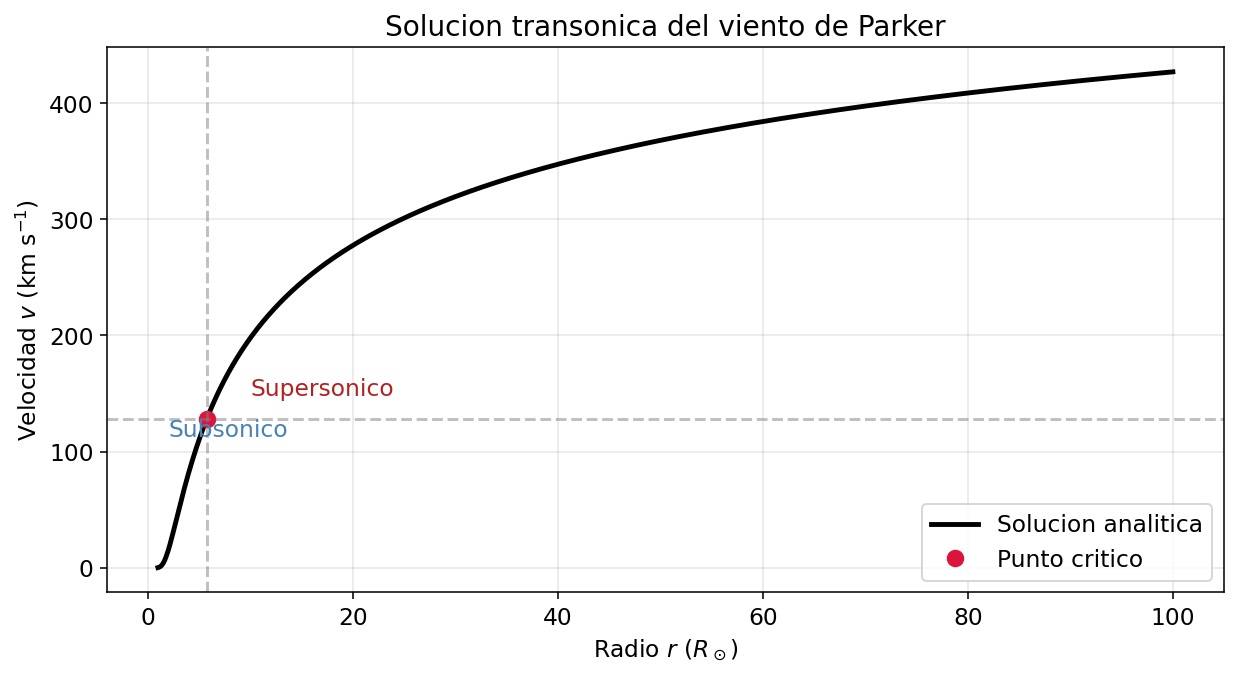
\includegraphics[width=\linewidth]{figuras/01_solucion_analitica.png}
    \column{0.40\textwidth}
      \footnotesize
      \begin{itemize}
        \item La curva cruza suavemente el punto s\'onico $(r_c,v_c)$, sin quiebres ni discontinuidades.
        \item A radios peque\~nos domina el r\'egimen subs\'onico: el plasma todav\'ia est\'a fuertemente ligado a la gravedad solar.
        \item Despu\'es del cruce, la pendiente positiva muestra que la presi\'on t\'ermica logra sostener una aceleraci\'on supers\'onica persistente.
        \item La gr\'afica confirma que la soluci\'on f\'isica no es est\'atica: el plasma debe escapar y ganar velocidad con el radio.
        \item Esta curva funciona como referencia para juzgar si los m\'etodos num\'ericos reproducen la transici\'on correcta.
      \end{itemize}
  \end{columns}
\end{frame}

\begin{frame}{Conservaci\'on de masa}
  Adem\'as de la ecuaci\'on de momento, el flujo cumple continuidad:
  \[
    \dot{M} = 4\pi r^2 \rho(r) v(r)
  \]

  \begin{itemize}
    \item En flujo estacionario, $\dot{M}$ es constante con el radio.
    \item Una vez obtenida la velocidad, la densidad se calcula directamente.
    \item Esto permite separar dos preguntas:
    \item La ecuaci\'on de momento fija la forma de $v(r)$.
    \item La continuidad fija cu\'anta masa corresponde a esa soluci\'on.
  \end{itemize}
\end{frame}

\begin{frame}{Parte num\'erica: integradores}
  \begin{block}{Euler expl\'icito}
    \[
      v_{n+1} = v_n + \left.\frac{dv}{dr}\right|_{r_n}\Delta r
    \]
  \end{block}

  \begin{block}{Runge-Kutta de cuarto orden}
    \[
      v_{n+1} = v_n + \frac{\Delta r}{6}\left(k_1 + 2k_2 + 2k_3 + k_4\right)
    \]
  \end{block}

  \begin{itemize}
    \item Euler es simple, pero acumula error y exige pasos m\'as peque\~nos.
    \item RK4 cuesta m\'as por paso, pero permite una trayectoria mucho m\'as precisa.
    \item En el proyecto se usan escalas t\'ipicas de $10^5$ m para Euler y $10^6$ m para RK4.
    \item La comparaci\'on es importante porque muestra el compromiso entre costo computacional y precisi\'on.
  \end{itemize}
\end{frame}

\begin{frame}{Tratamiento del punto cr\'itico}
  \begin{itemize}
    \item La ecuaci\'on diferencial se vuelve singular en $v=v_c$ porque aparece una forma $0/0$.
    \item El c\'odigo evita iniciar exactamente en ese punto.
    \item Se parte desde $r_c(1+\varepsilon)$ para la rama supers\'onica y desde $r_c(1-\varepsilon)$ para la subs\'onica.
    \item Luego se integran ambas ramas por separado y se unen en una soluci\'on continua.
    \item Este paso es clave: sin ese desplazamiento, la integraci\'on falla num\'ericamente.
  \end{itemize}
\end{frame}

\begin{frame}{Por qu\'e RK4 funciona mejor}
  \begin{itemize}
    \item Euler usa solo la pendiente local al inicio de cada paso.
    \item RK4 eval\'ua pendientes intermedias y construye un promedio ponderado m\'as fiel a la curvatura real de la soluci\'on.
    \item Cerca del punto s\'onico, la soluci\'on cambia de r\'egimen y el error local se propaga con rapidez.
    \item Por eso RK4 puede usar pasos mayores sin degradar la estabilidad de forma importante.
  \end{itemize}
\end{frame}

\begin{frame}{Comparaci\'on num\'erica}
  Error relativo frente a la referencia anal\'itica en $r=50\,R_\odot$:

  \begin{table}
    \centering
    \begin{tabular}{lc}
      \toprule
      M\'etodo & Error relativo \\
      \midrule
      RK4 & $1.39 \times 10^{-10}$ \\
      Euler & $1.58 \times 10^{-6}$ \\
      \bottomrule
    \end{tabular}
  \end{table}

  \begin{itemize}
    \item RK4 reproduce la curva trans\'onica con error pr\'acticamente despreciable.
    \item Euler conserva la tendencia correcta, pero es mucho m\'as sensible al tama\~no de paso.
    \item La diferencia de cuatro \'ordenes de magnitud justifica usar RK4 como m\'etodo principal del proyecto.
  \end{itemize}
\end{frame}

\begin{frame}{Comparaci\'on visual: Euler vs RK4}
  \begin{columns}[c]
    \column{0.58\textwidth}
      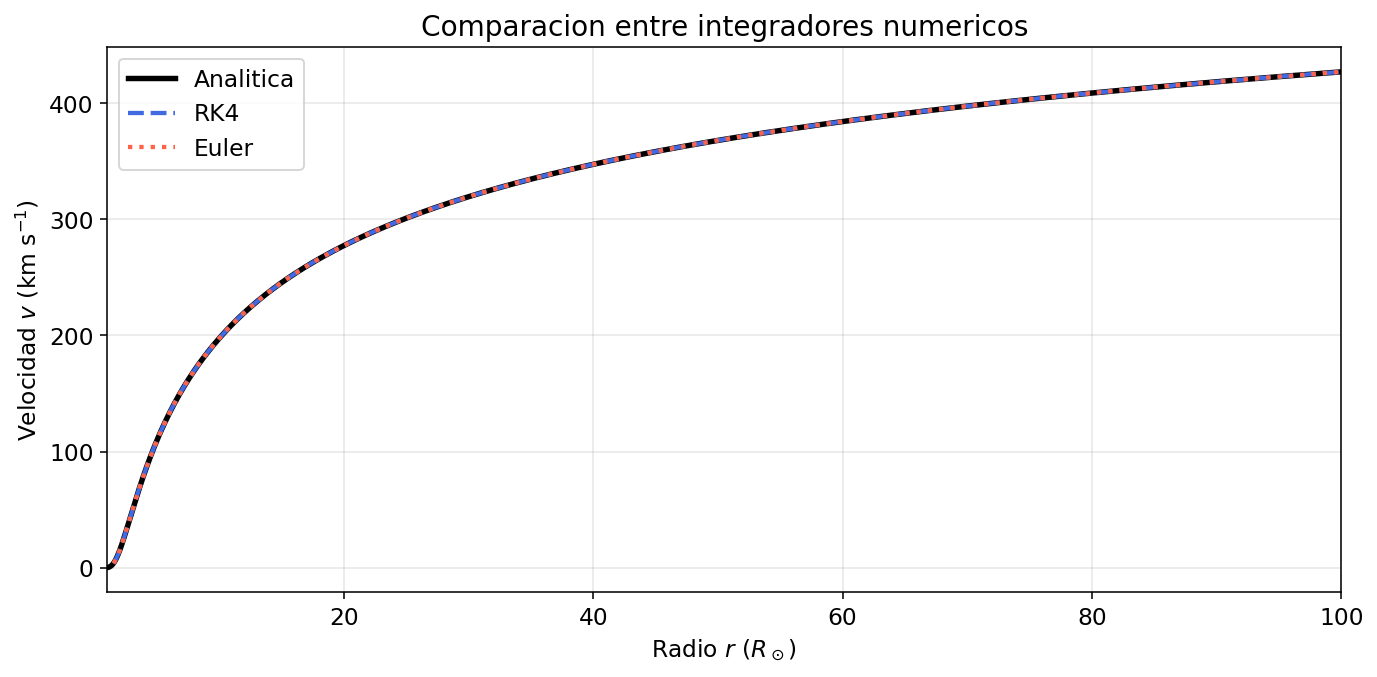
\includegraphics[width=\linewidth]{figuras/02_comparacion_metodos.png}
    \column{0.38\textwidth}
      \footnotesize
      \begin{itemize}
        \item RK4 queda pr\'acticamente superpuesto a la curva de referencia en todo el dominio.
        \item Euler tambi\'en acelera el flujo, pero se separa gradualmente porque arrastra el error local de cada paso.
        \item La discrepancia se vuelve m\'as visible lejos del punto inicial, donde los errores acumulados ya modifican la trayectoria.
        \item La lectura de la figura es num\'erica y f\'isica: ambos m\'etodos captan el mecanismo del viento, pero solo RK4 reproduce con precisi\'on la tasa real de aceleraci\'on.
      \end{itemize}
  \end{columns}
\end{frame}

\begin{frame}{Sensibilidad a la temperatura}
  \begin{table}
    \centering
    \begin{tabular}{ccc}
      \toprule
      $T$ [K] & $r_c\ [R_\odot]$ & $v(100R_\odot)$ [km/s] \\
      \midrule
      $5\times10^5$ & 11.55 & 260.1 \\
      $10^6$ & 5.78 & 426.9 \\
      $2\times10^6$ & 2.89 & 678.1 \\
      \bottomrule
    \end{tabular}
  \end{table}

  \begin{itemize}
    \item Al aumentar la temperatura, aumenta $v_c$.
    \item El punto s\'onico se acerca al Sol.
    \item El viento se acelera m\'as r\'apido y alcanza mayores velocidades terminales.
    \item Este resultado traduce una idea f\'isica simple: una corona m\'as caliente tiene mayor capacidad de impulsar el plasma.
  \end{itemize}
\end{frame}

\begin{frame}{Sensibilidad a la temperatura: perfiles}
  \begin{columns}[c]
    \column{0.60\textwidth}
      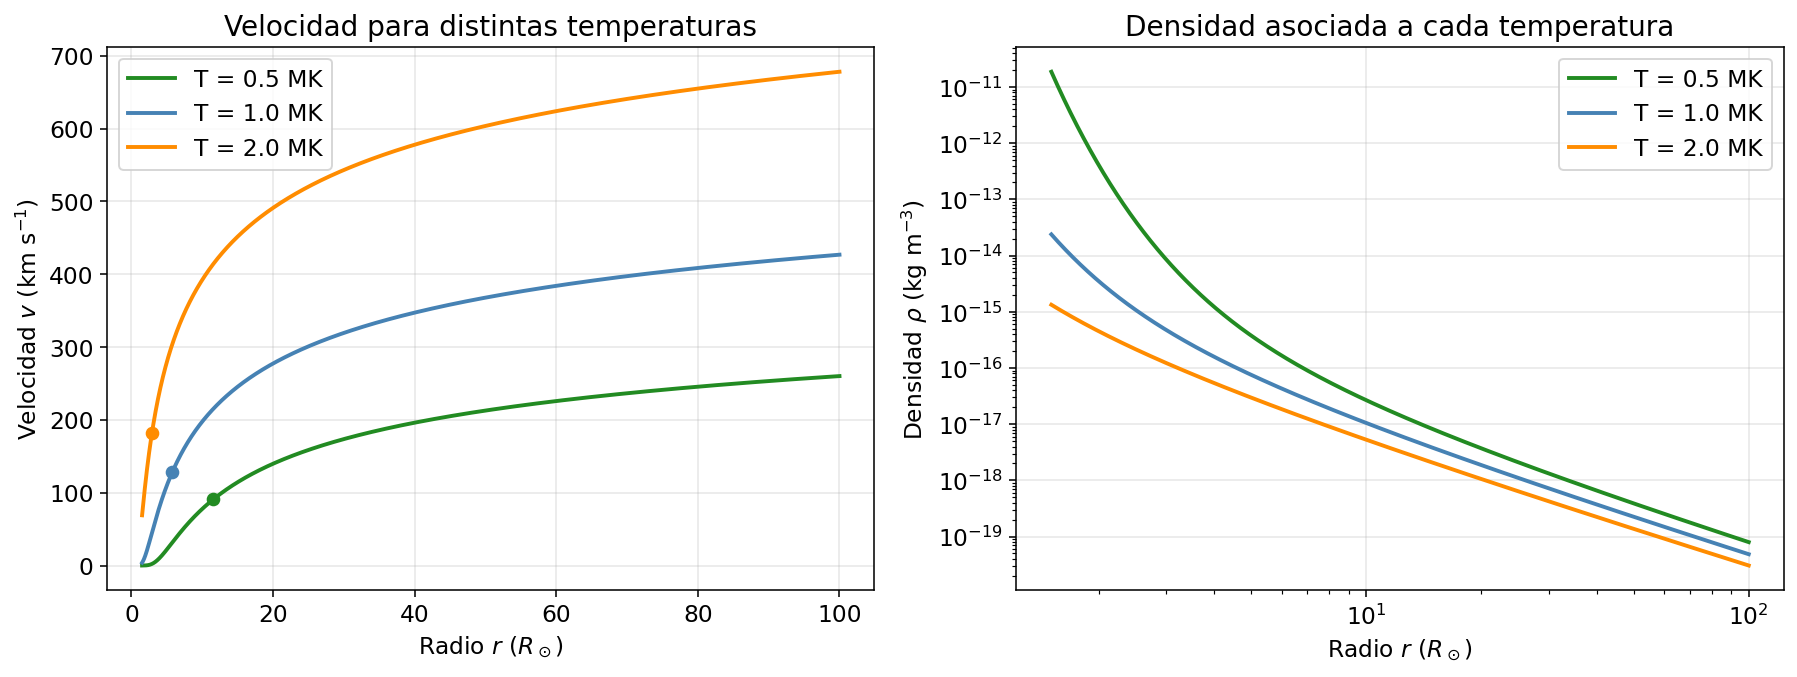
\includegraphics[width=\linewidth]{figuras/03_sensibilidad_temperatura.png}
    \column{0.36\textwidth}
      \footnotesize
      \begin{itemize}
        \item Las curvas de velocidad se ordenan con la temperatura: una corona m\'as caliente produce un viento m\'as r\'apido en casi todo radio.
        \item El cruce s\'onico ocurre antes cuando $T$ aumenta, por eso las curvas calientes entran m\'as r\'apido al r\'egimen supers\'onico.
        \item En densidad, las soluciones m\'as calientes caen con mayor rapidez porque el mismo flujo de masa se reparte en un plasma que acelera m\'as.
        \item La gr\'afica muestra que la temperatura no es un detalle de escala: controla directamente la estructura din\'amica del viento.
      \end{itemize}
  \end{columns}
\end{frame}

\begin{frame}{Flujo de masa y calentamiento}
  \begin{columns}[c]
    \column{0.60\textwidth}
      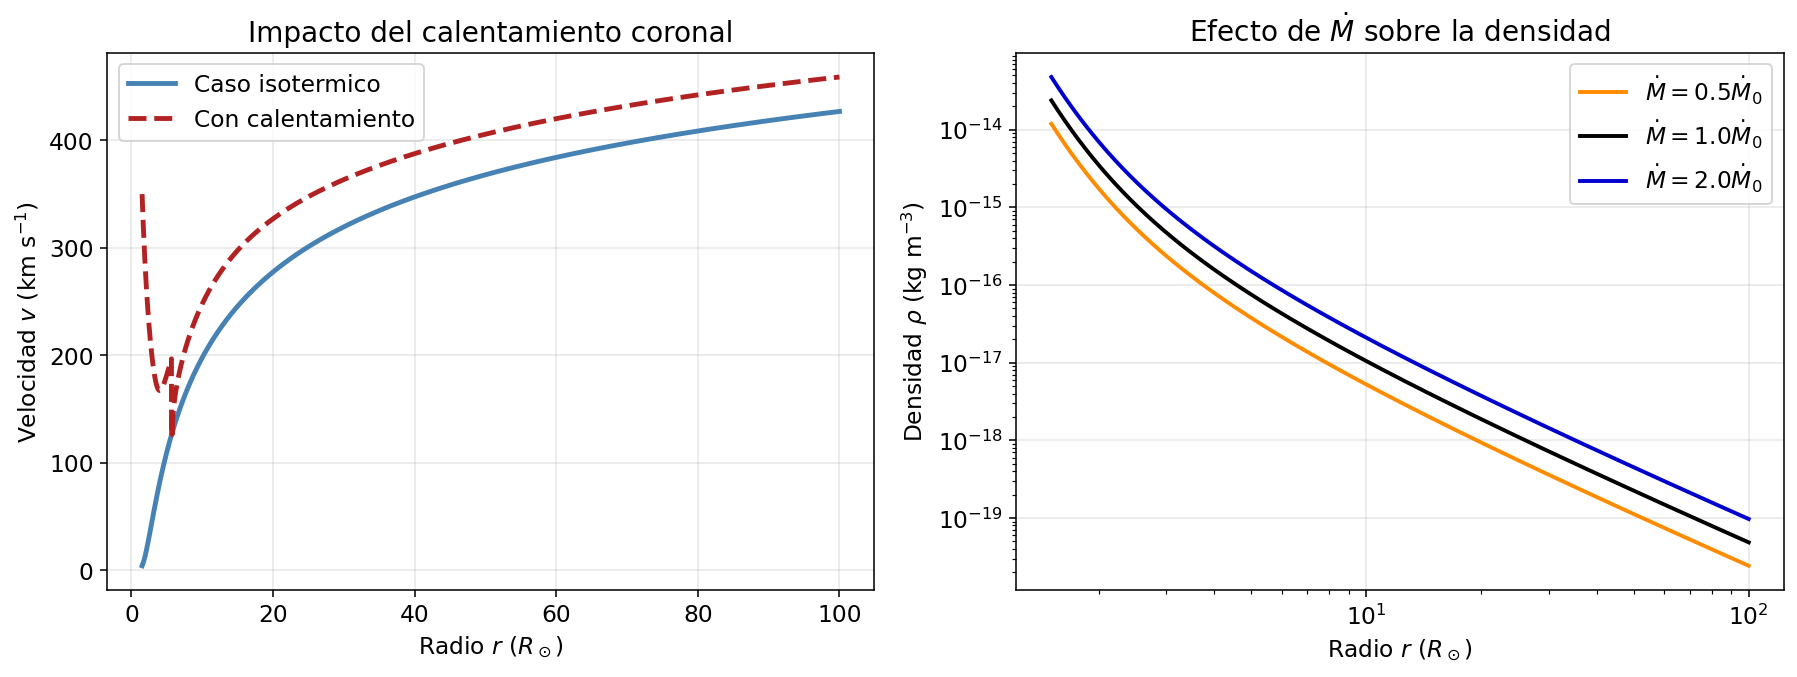
\includegraphics[width=\linewidth]{figuras/04_flujo_y_calentamiento.png}
    \column{0.36\textwidth}
      \footnotesize
      \begin{itemize}
        \item Las curvas asociadas a distintos $\dot{M}$ conservan casi la misma velocidad, pero cambian su nivel de densidad.
        \item Esto confirma que continuidad fija cu\'anta materia fluye, mientras que la ecuaci\'on de movimiento fija c\'omo se acelera.
        \item Cuando se agrega calentamiento, la curva de velocidad se eleva a grandes radios: hay m\'as energ\'ia disponible para vencer la gravedad.
        \item La lectura f\'isica es que densidad y aceleraci\'on no responden al mismo mecanismo, aunque aparezcan acopladas en el plasma real.
      \end{itemize}
  \end{columns}
\end{frame}

\begin{frame}{Lectura f\'isica de los resultados}
  \begin{itemize}
    \item El modelo muestra que no toda atm\'osfera caliente puede permanecer en equilibrio gravitacional.
    \item La soluci\'on trans\'onica es una consecuencia de consistencia matem\'atica y de plausibilidad f\'isica.
    \item La velocidad no depende directamente de $\dot{M}$, sino de la competencia entre temperatura y gravedad.
    \item La densidad s\'i depende de $\dot{M}$, porque continuidad fija cu\'anta materia fluye por cada esfera de radio $r$.
    \item Las gr\'aficas muestran que cada par\'ametro tiene una firma distinta: $T$ desplaza el punto s\'onico y cambia la aceleraci\'on, mientras $\dot{M}$ reescala principalmente la densidad.
    \item En conjunto, el proyecto conecta teor\'ia astrof\'isica, formulaci\'on anal\'itica y validaci\'on computacional.
  \end{itemize}
\end{frame}

\begin{frame}{Conclusiones}
  \begin{itemize}
    \item El proyecto reproduce la soluci\'on trans\'onica del viento solar de Parker.
    \item La estructura del c\'odigo est\'a separada con claridad entre constantes, referencia anal\'itica e integraci\'on num\'erica.
    \item El punto cr\'itico domina tanto la interpretaci\'on f\'isica como la estrategia computacional.
    \item RK4 resulta ser el m\'etodo m\'as robusto para este problema con singularidad aparente.
    \item La temperatura coronal controla la posici\'on del punto s\'onico y la velocidad final del viento.
  \end{itemize}
\end{frame}

\end{document}
